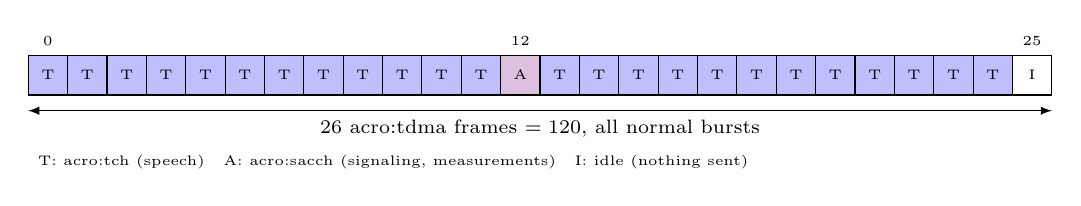
\begin{tikzpicture}[>=latex, x=0.5cm, y=1cm]
    % 26-multiframe of a full-rate traffic channel (one timeslot)
    \foreach \n in {0,...,25} {
        \ifnum\n=12 \def\lab{A}\def\col{violet!25}%
        \else\ifnum\n=25 \def\lab{I}\def\col{white}%
        \else \def\lab{T}\def\col{blue!25}%
        \fi\fi
        \draw[fill=\col] (\n,0) rectangle ++(1,0.5);
        \node[font=\tiny] at ({\n+0.5},0.25) {\lab};
    }
    \foreach \n in {0,12,25} {
        \node[font=\tiny, anchor=south] at ({\n+0.5},0.5) {\n};
    }
    \draw[<->] (0,-0.2) -- (26,-0.2)
        node[midway, below, font=\scriptsize] {26 \gls{acro:tdma} frames $=\qty{120}{\milli\second}$, all normal bursts};
    \node[font=\tiny, anchor=west] at (0,-0.85) {T: \acrshort{acro:tch} (speech)\quad A: \acrshort{acro:sacch} (signaling, measurements)\quad I: idle (nothing sent)};
\end{tikzpicture}
